\chapter{Method}
\label{chap:method}

The preceding chapters introduced the theoretical and methodological context required to describe OGAD. Chapter~\ref{chap:background} presented the graph foundations, the graph-generation problem, graphons, and graphon estimation, while Chapter~\ref{chap:related_works} reviewed the relevant graphon-estimation, graph-generation, diffusion, and evaluation methods. The purpose of this chapter is different: it specifies how these components are instantiated and connected in OGAD.

OGAD transforms a collection of observed finite graphs into a generator of new finite graphs through an intermediate graphon-derived representation. Training graphs are first processed by SIGL to obtain graphon estimates. These functions are evaluated on fixed finite grids and quantized into categorical tensors, over which a discrete diffusion model is trained. Generated categorical tensors are subsequently dequantized into probability-like graphon grids, from which finite graphs are sampled through Bernoulli edge draws. The resulting graph distributions are evaluated through the GGME pipeline and compared with direct graph-generation and classical probabilistic baselines.

\begin{figure}[H]
    \centering
    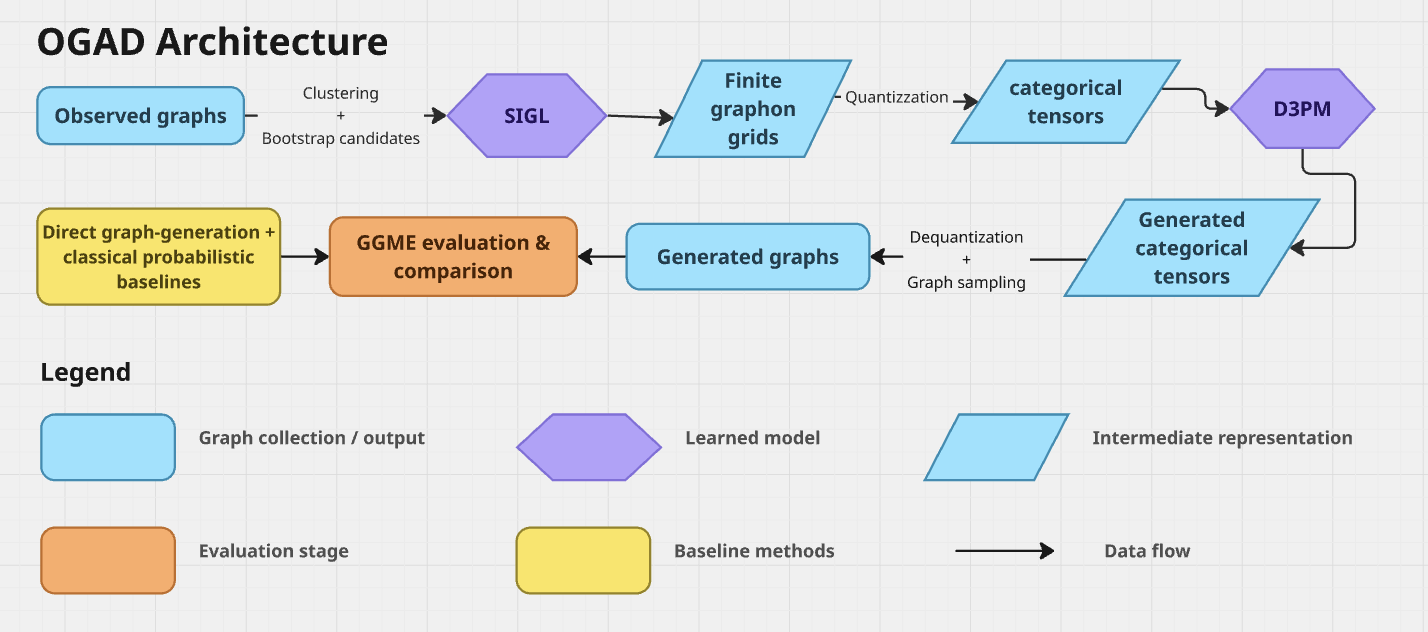
\includegraphics[width=\textwidth]{figures/method_overview.png}
    \caption{Overview of the OGAD architecture.}
    \label{fig:ogad_architecture}
\end{figure}

DA AGGIUNGERE UNA FIGURA ARCHITETTURALE E DEI PSEUDOCODICI PER FACILITARE LA RIPRODUCIBILITA' DELLO STUDIO.

\section{Method Overview}
\label{sec:method_overview}

At an abstract level, the OGAD pipeline can be represented as

\[
\mathcal{G}_{\mathrm{train}}
\longrightarrow
\left\{\widehat{W}^{(R)}_i\right\}
\longrightarrow
\left\{X_i\right\}
\longrightarrow
p_\theta(X)
\longrightarrow
\left\{\widetilde{W}_j\right\}
\longrightarrow
\left\{\widetilde{G}_j\right\},
\]

where \(\mathcal{G}_{\mathrm{train}}\) denotes the observed training graphs, \(\widehat{W}^{(R)}_i\) a finite numerical graphon estimate evaluated on an \(R\times R\) grid, \(X_i\) its categorical representation used by the diffusion model, \(p_\theta\) the learned distribution over such tensors, \(\widetilde{W}_j\) a generated probability-like grid after dequantization and post-processing, and \(\widetilde{G}_j\) a finite graph sampled from that grid.

The notation distinguishes three objects that play different roles:

\[
W
\neq
\widehat{W}^{(R)}
\neq
X.
\]

Here, \(W:[0,1]^2\rightarrow[0,1]\) is a mathematical graphon of the type introduced in Section~\ref{sec:graphons}; \(\widehat{W}^{(R)}\) is a finite numerical evaluation of an estimated graphon; and \(X\) is an integer-valued categorical tensor obtained by quantizing that finite grid. D3PM therefore operates neither on an arbitrary measurable graphon function nor directly on a binary graph, but on a fixed-dimensional categorical representation derived from an estimated graphon.

% TODO: Figure -- end-to-end OGAD methodological pipeline


\section{Input Graphs and Data Partitioning}
\label{sec:method_input_partitioning}

OGAD operates on finite simple undirected graphs represented by adjacency matrices, following the assumptions introduced in Section~\ref{sec:basic_graph_theory}. Input graphs are stored sparsely and converted to dense floating-point adjacency matrices before SIGL processing.

The pipeline uses two distinct validation mechanisms, operating on different representations and serving different purposes.

When GGME-based candidate selection is enabled, the original training set is first partitioned as

\[
\mathcal{G}_{\mathrm{train}}
=
\mathcal{G}_{\mathrm{model}}
\cup
\mathcal{G}_{\mathrm{GGME-val}},
\qquad
\mathcal{G}_{\mathrm{model}}
\cap
\mathcal{G}_{\mathrm{GGME-val}}
=
\varnothing.
\]

The thesis implementation uses an 80/20 split with random seed \(0\). Only $\mathcal{G}_{\mathrm{model}}$ is passed to graphon estimation. The held-out subset $\mathcal{G}_{\mathrm{GGME-val}}$ is reserved for the later graph-level comparison of trained D3PM candidates. When GGME-based candidate selection is disabled, all available training graphs are instead passed to graphon estimation.

After SIGL has produced the finite graphon dataset, a second split is performed. Let

\[
\mathcal{W}
=
\left\{
\widehat{W}^{(R)}_1,
\ldots,
\widehat{W}^{(R)}_{N_W}
\right\}
\]

denote the collection of estimated finite graphon grids. These samples are divided into

\[
\mathcal{W}
=
\mathcal{W}_{\mathrm{D3PM-train}}
\cup
\mathcal{W}_{\mathrm{D3PM-val}},
\]

again using an 80/20 split with seed \(0\). The validation subset
\(\mathcal{W}_{\mathrm{D3PM-val}}\) is used during diffusion-model fitting for early stopping and best-checkpoint identification within each candidate configuration.

The two validation sets therefore have different roles:

\[
\mathcal{G}_{\mathrm{GGME-val}}
\quad\text{and}\quad
\mathcal{W}_{\mathrm{D3PM-val}}.
\]

The former contains finite graphs and is used for graph-domain candidate selection; the latter contains graphon grids and is used during D3PM optimization. Neither participates in final model selection against the test set. The final test/reference graph set remains outside training and candidate selection and is accessed only during final evaluation, including to provide the empirical node-count distribution used for final graph sampling.


\section{Graphon Estimation with SIGL}
\label{sec:method_sigl}

OGAD estimates graphons using Scalable Implicit Graphon Learning (SIGL), introduced by Azizpour, Zilberstein, and Segarra \cite{azizpour2025scalable}. The general graphon-estimation problem was introduced in Section~\ref{sec:graphon_estimation}, while SIGL and related estimators were reviewed in Section~\ref{sec:rw_graphon_estimation}. This section therefore focuses on the specific procedure instantiated by OGAD.

\subsection{Clustering and Bootstrap Construction}
\label{subsec:method_sigl_clustering}

Clustering and bootstrapping serve distinct but complementary purposes in the construction of the graphon-estimation jobs. Clustering restricts each job to a subset of structurally related graphs, rather than combining graphs with potentially different structural characteristics, while bootstrap resampling produces multiple finite samples from each such subset.

When clustering is enabled, the graphs in $\mathcal{G}_{\mathrm{model}}$ are first represented using structural information derived from their degree distributions, local clustering coefficients, and normalized-Laplacian spectra. These descriptors were introduced in Sections~\ref{subsec:degree_density}, \ref{subsec:clustering_coefficient}, and~\ref{subsec:laplacian_spectrum}. The resulting feature vectors are standardized before KMeans clustering is applied.

Let \(C_{\mathrm{req}}\) denote the requested number of clusters. Only cluster labels containing graphs are retained, so the effective number of clusters may satisfy
\[
C_{\mathrm{eff}}
\leq
C_{\mathrm{req}}.
\]

Bootstrap resampling is then performed independently within every non-empty cluster. For a cluster containing \(n_c\) graphs, one bootstrap replicate draws \(n_c\) graph indices with replacement and uses the resulting collection as one SIGL estimation job.

Let \(B_{\mathrm{boot}}\) denote the configured number of bootstrap replicates per effective cluster. In the clustered configuration used in the thesis, the original unresampled cluster collections are not additionally included. Since \(B_{\mathrm{boot}}>1\) in these executions, the resulting number of graphon-estimation jobs is
\[
N_W
=
C_{\mathrm{eff}}B_{\mathrm{boot}}.
\]

This relation describes the instantiated clustered-bootstrap configuration rather than a general property of SIGL. When clustering is disabled, the implementation instead constructs one graphon-estimation job per model-training graph.

\subsection{One Graphon-Estimation Job}
\label{subsec:method_sigl_job}

Within each SIGL job, a graph convolutional network predicts one scalar coordinate per node from random scalar node features. The features are processed through GCN layers with ReLU activations followed by a scalar projection, sigmoid activation, and within-graph min--max normalization. Nodes are then sorted according to the resulting coordinates, and the induced permutation is applied consistently to the rows and columns of the corresponding adjacency matrix.

This ordering is learned independently within each estimation job and should not be interpreted as defining one global coordinate alignment across graphons estimated from different clusters or bootstrap samples.

The reordered adjacency matrices are average-pooled. Let

\[
\widehat{H}_g
\in
\mathbb{R}^{k_g\times k_g}
\]

denote the pooled representation associated with graph \(g\). In the implementation, pooled cells are associated with midpoint coordinates

\[
u_{g,i}
=
\frac{i+\tfrac{1}{2}}{k_g},
\qquad
v_{g,j}
=
\frac{j+\tfrac{1}{2}}{k_g},
\]

for

\[
i,j\in\{0,\ldots,k_g-1\}.
\]

Thus each pooled cell supplies a coordinate--value observation

\[
\left(
u_{g,i},
v_{g,j},
\widehat{H}_g(i,j)
\right)
\]

for the final implicit graphon regression.

As reviewed in Section~\ref{subsec:rw_neural_graphon_estimators}, the original SIGL formulation fits the final implicit representation from pooled coordinate--value observations. In the OGAD implementation, observations contributed by each graph are additionally weighted according to graph size. If graph \(g\) contains \(n_g\) nodes, its graph-level weight is

\[
w_g
=
\frac{n_g}
{\sum_h n_h},
\]

where the denominator is the total number of nodes contributed by the graphs in the current estimation job.

The final representation is a SIREN-style multilayer perceptron with sinusoidal hidden activations \cite{sitzmann2020implicit} and a sigmoid output. The architectural widths were not tuned in this work, but inherited from the reference SIGL implementation: the coordinate-prediction GCN uses hidden dimensions \(8,8,8\), while the SIREN graphon model uses \(20,20\). These values were kept fixed throughout the experiments.
Once fitted, the implicit function is evaluated on a regular midpoint grid. For

\[
r,s\in\{0,\ldots,R-1\},
\]

define

\[
u_r
=
\frac{r+\tfrac{1}{2}}{R},
\qquad
v_s
=
\frac{s+\tfrac{1}{2}}{R}.
\]

If \(f_{\theta^\star}\) denotes the fitted implicit representation, its finite evaluation is

\[
\widehat{W}^{(R)}_{rs}
=
f_{\theta^\star}(u_r,v_s),
\]

yielding

\[
\widehat{W}^{(R)}
\in
[0,1]^{R\times R}.
\]

Before persistence, the grid is symmetrized,

\[
\widehat{W}^{(R)}
\leftarrow
\frac{
\widehat{W}^{(R)}
+
\widehat{W}^{(R)\top}
}{2},
\]

and its diagonal is set to zero. In the thesis executions,

\[
R=128.
\]

This value was chosen as a practical trade-off between preserving sufficient spatial detail in the estimated graphon and keeping the subsequent D3PM training computationally feasible within the available GPU memory. 
The resulting \(128\times128\) matrix is the interface between the continuous implicit graphon estimate and the subsequent fixed-dimensional generative model.


\section{Finite Graphon Representation and Discretization}
\label{sec:method_graphon_discretization}

The transition from SIGL to D3PM introduces the central representational change of OGAD:

\[
W
\longrightarrow
\widehat{W}^{(R)}
\longrightarrow
X.
\]

The distinction between a mathematical graphon and a finite numerical graphon representation was introduced in Section~\ref{subsec:numerical_graphon_representation}. OGAD additionally maps the finite grid into a categorical state space.

The estimated graphon grids are persisted as grayscale images and subsequently reloaded as normalized single-channel tensors. This serialization step does not alter their intended interpretation as finite edge-probability representations. Each D3PM input has shape

\[
[1,R,R],
\]

which becomes

\[
[1,128,128]
\]

in the thesis implementation.

Let

\[
\widehat{W}^{(R)}_{ij}\in[0,1]
\]

denote one value of the reloaded finite graphon tensor, and let \(K\) be the number of categorical states used by a D3PM candidate. OGAD applies the element-wise quantization operator

\[
\mathcal{Q}_K
\left(
\widehat{W}^{(R)}_{ij}
\right)
=
\operatorname{clamp}
\left(
\operatorname{round}
\left(
(K-1)\widehat{W}^{(R)}_{ij}
\right),
0,
K-1
\right).
\]

The resulting categorical state is

\[
X_{ij}
=
\mathcal{Q}_K
\left(
\widehat{W}^{(R)}_{ij}
\right)
\in
\{0,\ldots,K-1\},
\]

and element-wise quantization produces

\[
X
\in
\{0,\ldots,K-1\}^{1\times R\times R}.
\]

Thus the mathematical graphon itself has not become discrete. A finite numerical representation has instead been encoded in the categorical state space required by D3PM.


\section{Discrete Diffusion over Graphon Representations}
\label{sec:method_d3pm}

OGAD models the categorical graphon tensors using the D3PM framework introduced by Austin et al.~\cite{austin2021structured}. The general categorical diffusion formulation was reviewed in Section~\ref{subsec:rw_discrete_graph_diffusion}; the present section specifies the state space, transition process, denoising architecture, and objective instantiated in OGAD.

For one graphon sample,

\[ X_0 \in \{0,\ldots,K-1\}^{1\times R\times R}. \]

Each spatial position is therefore a categorical random variable with \(K\) possible states. Following the reference D3PM configuration for image generation \cite{austin2021structured}, OGAD uses

\[
T=1000
\]

diffusion steps. This value was kept fixed throughout the experiments rather than treated as an additional hyperparameter. The transition schedule is precomputed for \(T=1000\), while the implemented training and reverse-sampling loops operate over

\[
t\in\{1,\ldots,T-1\}.
\]

OGAD uses a uniform categorical forward process shared across all grid locations.

\subsection{Forward Process}
\label{subsec:method_d3pm_forward}

The corruption strength follows the cosine-derived schedule implemented by the D3PM component. For $t=0,\ldots,T,$ define $s_t = \frac{t}{T},$ and

\[
a_t
=
\cos
\left(
\frac{s_t+0.008}{1.008}
\frac{\pi}{2}
\right).
\]

For $t=1,\ldots,T,$ the transition strength is

\[
\beta_t
=
\min
\left(
1-\frac{a_t}{a_{t-1}},
0.999
\right).
\]

Given \(K\) categories, the one-step transition matrix $Q_t\in[0,1]^{K\times K}$ is

\[
Q_t(i,j)
=
\begin{cases}
\dfrac{\beta_t}{K},
&
i\neq j,
\\[6pt]
1-\dfrac{(K-1)\beta_t}{K},
&
i=j.
\end{cases}
\]

Each row therefore defines a categorical probability distribution. The cumulative transition matrix is

\[
\overline{Q}_t
=
Q_1Q_2\cdots Q_t.
\]

For a clean categorical value \(x_0\), the forward marginal at timestep \(t\) is obtained from the corresponding row of \(\overline{Q}_t\):

\[
q(x_t\mid x_0)
=
\operatorname{Cat}
\left(
x_t;
\overline{Q}_t[x_0,:]
\right).
\]

The same transition matrices are applied independently at every graphon-grid position.

Although the complete schedule is defined up to \(T\), the implemented training procedure samples timesteps uniformly from

\[
t\in\{1,\ldots,T-1\}
=
\{1,\ldots,999\}.
\]

The corrupted categorical tensor \(X_t\) is then sampled from the forward marginal using the cumulative matrix \(\overline{Q}_t\).


\subsection{Denoising Network}
\label{subsec:method_d3pm_network}

The clean-state predictor used by OGAD is the \texttt{DiT\_Llama} architecture. The model divides the input graphon representation into small spatial patches and processes them through a sequence of Transformer blocks conditioned on the diffusion timestep \(t\). Given the current categorical tensor \(X_t\), the network predicts categorical logits for the clean state \(X_0\).

The instantiated model uses one input channel, hidden dimension \(512\), patch size \(2\), five Transformer blocks, and sixteen attention heads. For a \(128\times128\) input, the \(2\times2\) patch decomposition produces

\[
\frac{128}{2}
\times
\frac{128}{2}
=
64\times64
=
4096
\]

spatial tokens. After embedding, the principal representation flow is

\[
[B,1,128,128]
\longrightarrow
[B,4096,512]
\longrightarrow
[B,1,128,128,K].
\]

The transformer uses timestep conditioning, rotary positional information, and adaptive normalization. The implementation also introduces a gated residual contribution based on a one-hot representation of the current noisy state \(X_t\).

The semantic prediction target is therefore

\[
\widehat{p}_\theta
\left(
X_0
\mid
X_t,t
\right).
\]

The network does not predict Gaussian noise and does not directly parameterize \(X_{t-1}\); it predicts logits for the original clean categorical tensor.


\subsection{Reverse Model and Training Objective}
\label{subsec:method_d3pm_objective}

Uppercase \(X_t\) denotes the complete categorical graphon tensor at timestep \(t\), whereas lowercase \(x_t\) denotes the categorical state at one individual grid position.

The clean-state probabilities predicted by the network are converted into reverse-transition probabilities using the known categorical forward process.
At one grid position, let

\[
\widehat{\pi}_\theta
=
\operatorname{softmax}
\left(
f_\theta(x_t,t)
\right)
\]

denotes the predicted probability distribution over the original clean state \(x_0\).
Each component \(\widehat{\pi}_{\theta,k}\) estimates the probability that the original state was category \(k\), given \(x_t\) and timestep \(t\).

For \(t>1\), define the unnormalized reverse-probability vector

\[
r_\theta(\cdot\mid x_t)
=
Q_t^\top[x_t,:]
\odot
\left(
\widehat{\pi}_\theta
\overline{Q}_{t-1}
\right),
\]

where \(Q_t^\top[x_t,:]\) denotes the row indexed by the observed category \(x_t\) in \(Q_t^\top\), equivalently the \(x_t\)-th column of \(Q_t\), and \(\odot\) denotes element-wise multiplication.

The normalized reverse distribution is

\[
p_\theta
\left(
x_{t-1}=k
\mid
x_t
\right)
=
\frac{
r_{\theta,k}(\cdot\mid x_t)
}{
\sum_{\ell=0}^{K-1}
r_{\theta,\ell}(\cdot\mid x_t)
}.
\]

The quantity \(p_\theta(x_{t-1}=k\mid x_t)\) therefore represents the normalized reverse-transition probability that the previous state is category \(k\), given the current state \(x_t\). It is obtained by normalizing \(r_\theta(\cdot\mid x_t)\) over all \(K\) categories.
The implementation performs this computation in log space for numerical stability. For \(t=1\), the posterior construction is replaced by the predicted \(x_0\) logits themselves.

Training uses

\[
\mathcal{L}
=
\mathcal{L}_{\mathrm{vb}}
+
\lambda
\mathcal{L}_{\mathrm{CE}},
\]

where \(\lambda\) is the configured hybrid-loss coefficient.

Let \(\ell\) index all categorical positions after flattening the batch and spatial dimensions, and let \(N\) denote their total number. The implemented variational component is the mean posterior KL divergence

\[
\mathcal{L}_{\mathrm{vb}}
=
\frac{1}{N}
\sum_{\ell=1}^{N}
D_{\mathrm{KL}}
\left(
q_\ell
\left(
x_{t-1}
\mid
x_t,x_0
\right)
\;\middle\Vert\;
p_{\theta,\ell}
\left(
x_{t-1}
\mid
x_t
\right)
\right).
\]

The auxiliary clean-state term is the mean categorical cross-entropy,

\[
\mathcal{L}_{\mathrm{CE}}
=
-\frac{1}{N}
\sum_{\ell=1}^{N}
\log
\widehat{\pi}_{\theta,\ell}
\left(
x_{0,\ell}
\right).
\]

No additional timestep-dependent weighting is applied to these terms in the implementation.

Optimization is performed with AdamW. Learning-rate grids, candidate-specific values of \(\lambda\), batch size, epoch limits, and selected dataset-specific hyperparameters are reported with the experimental configuration.


\section{D3PM Training and Candidate Selection}
\label{sec:method_d3pm_selection}

OGAD distinguishes between checkpoint selection within one D3PM candidate and generator selection across candidate configurations.

For each candidate, training uses

\[
\mathcal{W}_{\mathrm{D3PM-train}},
\]

while the objective on

\[
\mathcal{W}_{\mathrm{D3PM-val}}
\]

is monitored for early stopping. The checkpoint achieving the best validation loss is retained for that candidate.

Each retained checkpoint is subsequently used to generate sixteen graphon-like tensors. When GGME-based candidate selection is enabled, these tensors are converted into finite graphs according to Section~\ref{sec:method_graph_sampling} and compared with

\[
\mathcal{G}_{\mathrm{GGME-val}}.
\]

Candidate selection therefore follows two levels:

\[
\text{best checkpoint within candidate}
\longrightarrow
\text{best generator across candidates}.
\]

The first level evaluates the diffusion objective on held-out graphon representations. The second evaluates the structural distribution of finite graphs generated by each candidate. Consequently, the generator selected through GGME need not coincide with the candidate having the lowest validation loss across the complete D3PM hyperparameter search.

The final test/reference graphs do not participate in either operation.


\section{Sampling Graphon-Like Representations}
\label{sec:method_d3pm_sampling}

Candidate graphon generation is initialized from independent uniform categorical noise. At every grid position,

\[
X_{\mathrm{init}}(i,j)
\sim
\operatorname{Uniform}
\{0,\ldots,K-1\}.
\]

With \(T=1000\), the reverse loop runs through

\[
t=T-1,T-2,\ldots,1
\]

or equivalently

\[
t=999,998,\ldots,1.
\]

The implementation initializes a batch of sixteen tensors in this way. At every intermediate step, the network predicts clean-state logits, these are converted into posterior logits for \(x_{t-1}\), and the next categorical state is sampled through categorical Gumbel-max sampling. At \(t=1\), no additional Gumbel noise is introduced, so the update becomes an argmax over the final logits. No temperature parameter is used.

The final categorical states are mapped back to numerical values through the dequantization operator

\[
\mathcal{D}_K(k)
=
\frac{k}{K-1},
\qquad
k\in\{0,\ldots,K-1\}.
\]

Before symmetry enforcement, the possible numerical values therefore belong to

\[
\left\{
0,
\frac{1}{K-1},
\ldots,
1
\right\}.
\]

Each generated matrix is then symmetrized,

\[
\widetilde{W}
\leftarrow
\frac{
\widetilde{W}
+
\widetilde{W}^{\top}
}{2},
\]

clipped to \([0,1]\), and assigned a zero diagonal.

Symmetrization can produce probabilities that do not belong to the original dequantization set. Consequently, the final object is more accurately described as a generated graphon-like probability grid:

\[
\widetilde{W}_j
\in
[0,1]^{R\times R}.
\]


\section{From Generated Graphons to Finite Graphs}
\label{sec:method_graph_sampling}

The graphon sampling principle was introduced in Section~\ref{subsec:graphon_sampling}. OGAD applies its finite-grid counterpart to generated probability matrices rather than interpreting those matrices directly as adjacency matrices.

Let

\[
\widetilde{W}
\in
[0,1]^{R\times R}
\]

be one sanitized generated grid. The number of graph nodes \(M\) is sampled from the empirical node-count distribution of the reference split used at the current stage. During GGME candidate selection this distribution is obtained from

\[
\mathcal{G}_{\mathrm{GGME-val}},
\]

while during final evaluation it is obtained from the final test/reference set. If a sampled node count exceeds \(R\), the implementation resamples until

\[
M\leq R.
\]

Thus, graph size is conditioned on the empirical reference distribution and is not independently generated by D3PM.

For each generated node \(i\),

\[
U_i
\sim
\mathcal{U}(0,1),
\]

and its latent value is mapped to the finite graphon-grid index

\[
z_i
=
\min
\left(
R-1,
\left\lfloor RU_i \right\rfloor
\right).
\]

The indices \(z_i\) are sampled independently with replacement.

For every unordered pair \(i<j\),

\[
P_{ij}
=
\widetilde{W}_{z_i,z_j},
\]

and the edge is sampled as

\[
A_{ij}
\sim
\operatorname{Bernoulli}
\left(
P_{ij}
\right).
\]

The binary adjacency matrix is completed by

\[
A_{ji}=A_{ij},
\qquad
A_{ii}=0.
\]

No interpolation or thresholding of the generated grid is performed, and no connectivity-enforcing post-processing is applied. Disconnected graphs and isolated nodes are therefore retained if they arise from the Bernoulli sampling procedure.

For a requested collection of \(N_G\) finite graphs, let

\[
s\in\{0,\ldots,N_G-1\}
\]

denote the zero-based graph-sample index. Since each selected D3PM candidate provides sixteen graphon-like tensors, sample \(s\) uses tensor index

\[
s\bmod 16.
\]

The tensors are therefore reused cyclically when \(N_G>16\).


\section{Evaluation and Model-Selection Integration}
\label{sec:method_ggme}

The motivation for distributional graph evaluation and the structural descriptors used throughout the thesis were introduced in Section~\ref{subsec:structural_fidelity} and Section~\ref{sec:basic_graph_theory}. MMD-based evaluation and its limitations were reviewed in Section~\ref{subsec:rw_structural_evaluation}.  This section specifies how OGAD instantiates this evaluation through three descriptor families: node-degree distributions, local clustering-coefficient distributions, and normalized-Laplacian spectral distributions.

Clustering coefficients and normalized-Laplacian spectra are represented by \(200\)-bin histograms over \([0,1]\) and \([0,2]\), respectively, while degree histograms retain data-dependent support. Histograms are density-normalized, and variable-length descriptors are padded before kernel evaluation.

Generated and reference graph sets are compared using exact MMD with linear or Gaussian kernels, with Gaussian bandwidths \(\sigma\in{0.1,1,10}\). Kernel calibration applies \texttt{AddEdges} perturbations from \(0.15\) to \(0.95\) in increments of \(0.05\), using seed \(42\), and selects the configuration according to the Pearson correlation between perturbation strength and discrepancy.

GGME is used both for D3PM candidate selection and final evaluation. During selection, each retained candidate is evaluated against \(\mathcal{G}_{\mathrm{GGME-val}}\), and the resulting discrepancies determine the selected candidate according to the configured rule. The selected model is then evaluated separately against the test/reference set; these final test MMD values are reported only as evaluation results and do not influence model selection.
